\chapter{Modelos de Regresión Bayesianos}

Parafraseando a \textcite[15-16]{DraperSmith98}, al realizar un análisis estadístico sobre algún fenómeno que presenta variabilidad, muchas veces lo que se busca es explorar los efectos que algunas \textit{variables explicativas} ejercen--- o parecen ejercer--- sobre una \textit{variable de interés}. En algunos casos puede darse que, efectivamente, exista una relación funcional simple entre ambos tipos de variables. No obstante es mucho más común que, o bien la relación sea mucho más compleja de lo que podemos entender o describir, o bien simplemente nos es desconocida. En ambos casos, lo que podemos hacer es \textit{modelar}--- esto es, aproximar--- esta relación mediante algunas funciones matemáticas. Por razones históricas relacionadas con el trabajo de Sir Francis Galton esta clase de modelos se conocen como \textit{modelos de regresión} \parencite[28]{Zepeda15}. 

\section{Regresión lineal} 
 
En el caso más sencillo, podemos pensar que $y=f(x)$. Sin embargo, en la mayoría de los casos este modelo tomado literalmente podría parecernos una mala aproximación. Pensemos en el caso en el que se busca describir el peso en kilogramos de una persona a partir de la estatura. Es claro que a una misma estatura le podrían corresponder distintos valores de peso. Así pues, la relación no puede ser completamente descrita solo por una función de la estatura. A pesar de ello, podemos observar empíricamente que a mayor estatura \textit{esperamos} un mayor peso. Esto nos llevaría a pensar que podemos modelar el \textit{valor esperado} de nuestra variable de interés mediante alguna función de las variables explicativas.\\

Esto quiere decir, bajo una perspectiva bayesiana paramétrica, que modelaremos la incertidumbre producto de la variabilidad en la variable de interés $Y$ mediante una distribución de probabilidad condicional $p(Y|\theta,X)$ cuyo valor esperado esté relacionado con las variables explicativas $X$ mediante una función $h(\theta,X)$ que depende también de ciertos parámetros $\theta$: 
\begin{equation} \label{eq:regr_gral}
Y|\theta,X \sim p(Y|\theta,X) \qquad E[Y|\theta,X] = h(\theta,X)
\end{equation} 
Las formas más simples de la función $h(\theta,X)$ son \textit{lineales en los coeficientes}, esto es de la forma siguiente 
\begin{equation*}
h(\theta,X) = \beta_0 + \beta_1X_1 + \beta_2X_2 + \dots + \beta_pXp, 
\end{equation*}
para $p$ variables explicativas\footnote{Las variables explicativas pueden llegar a ser transformaciones unas de otras como cuando se buscan ajustar relaciones de orden cuadrático o como cuando se incluyen interacciones.} y donde $\theta = (\beta_0,\beta_1,\dots,\beta_p,\theta_r)$ con $\theta_r$ posibles parámetros adicionales de la distribución condicional de $Y$ dado $X$ pero que no determinan su esperanza.\\

Debido a que no conocemos la verdadera relación entre nuestras variables, tenemos incertidumbre sobre los valores de los coeficientes que determinan nuestra función $h(\theta ,X)$. Así pues, bajo la perspectiva bayesiana debemos reflejar dicha incertidumbre también mediante alguna distribución de probabilidad $p(\theta)$. Buscaremos, entonces, reducir esta incertidumbre mediante la recolección de datos $(y,x)$ que nos permitan, a través del teorema de Bayes obtener la distribución posterior $p(\theta|y,x)$.\\

Como bien notan tanto \textcite[354]{Gelman13} como \textcite[111]{Congdon06}, el modelo más general debería incorporar también la incertidumbre que pudiera existir sobre las variables explicativas $X$ derivada, por ejemplo, de posibles errores de medición. Sin embargo, si se puede asumir que los parámetros $\varphi$ de la distribución marginal de $X$, $p(X|\varphi)$, son independientes de $\theta$--- es decir $p(\varphi,\theta)=p(\varphi)p(\theta)$--- al aplicar el Teorema de Bayes veríamos que la distribución posterior $p(\theta|y,x)$ no dependería de $\varphi$ por lo que podemos proceder ignorando dicha incertidumbre para efectos de las inferencias sobre $\theta$. Por eso--- y para simplificar la notación--- en lo que sigue omitiré la condicional en $X$, con lo que $p(\theta|y,x)$ se convierte en $p(\theta|y)$, por ejemplo. \\

El modelo de regresión más usual es cuando se asume que la variable de interés depende linealmente de las variables explicativas salvo por un error aleatorio que se distribuye normal. Esto es, supongamos que tenemos $N$ conjuntos de observaciones, condicionalmente independientes, $\left\lbrace(y_i,x_{i,1},\dots,x_{i,p-1})\right\rbrace_{i=1}^{N}$ donde nuestra variable de interés es $Y$ y contamos con $p-1$ variables explicativas $\left\lbrace X_j\right\rbrace_{j=1}^{p-1}$, la regresión lineal normal bajo los supuestos usuales es: 
\begin{align*} 
y_i = \beta_0 + \beta_1 x_{i,1} + \dots + \beta_{p-1} x_{i,p-1} + \epsilon_i \qquad \epsilon_i \sim N(0,\sigma^2) \quad \forall i = 1,\dots, N. 
\end{align*}
Que en términos de la \textbf{Ecuación \ref{eq:regr_gral}} sería
\begin{equation}
y_i|\theta \sim N(\mu_i,\sigma^2) \quad \mu_i = E[y_i|\theta] = \beta x_i \quad \forall i = 1, \dots, N,
\end{equation}
donde $\beta = (\beta_0,\beta_1,\dots,\beta_{p-1})$, $x_i = (1,x_{i,1},\dots,x_{i,p-1})$ y tal que  $\theta = (\beta,\sigma^2)$ tenga alguna distribución inicial apropiada.\\ 

También es posible aprovechar la notación matricial para simplificar estas expresiones, así como trabajar con ellas. Definiendo lo siguiente,  
\begin{align*}
X &= 
\begin{pmatrix}
  1 & x_{1,1} & \cdots & x_{1,p-1} \\
  \vdots & \vdots & \ddots & \vdots  \\
  1 & x_{N,1} & \cdots & x_{N,p-1} 
\end{pmatrix} \in \mathbb{R}_{N\mathsf{x}p}, \\
y &= (y_1,\dots,y_N)^T \in \mathbb{R}_{N\mathsf{x}1},\\
\beta &= (\beta_0,\beta_1,\dots,\beta_{p-1})^T \in \mathbb{R}_{p\mathsf{x}1}, 
\end{align*}
tenemos que el modelo de regresión normal puede ser expresado de manera compacta de la siguiente forma: 
\begin{equation}\label{eq:modelo_normal_matricial}
y|\theta \sim N_N(X\beta,\sigma^2\mathbb{I}_N) \quad \text{tal que} \quad \theta = (\beta, \sigma^2) \sim p(\beta,\sigma^2), 
\end{equation} 
donde $N_N(X\beta,\sigma^2\mathbb{I}_N)$ representa una distribución normal $N-$variada con media $X\beta$ y varianzas individuales $\sigma^2$ y $p(\beta,\sigma^2)$ una distribución inicial para los parámetros desconocidos. 

\subsection{Análisis bayesiano del modelo lineal normal}

Ahora bien, para realizar un análisis bayesiano del modelo requerimos especificar una distribución inicial para $\theta$ y, mediante el teorema de Bayes, actualizarla para obtener una distribución posterior dados los datos observados. Entonces, primero presento una manipulación de la función de verosimilitud para después ver algunas distribuciones iniciales frecuentemente utilizadas y, finalmente, realizar la actualización de las mismas dados los datos. 

\subsubsection*{Verosimilitud}

Siguiendo a \textcites[Cap. 3]{GP98}[Sec. 4.2 ]{Congdon06}, manipulemos la función de verosimilitud de la normal multivariada de la \textbf{Ecuación \ref{eq:modelo_normal_matricial}} para facilitar la actualización mediante el teorema de Bayes. Observemos que:
\begin{align}\label{eq:modelo_normal_prop}
p(y|\theta) &= \dfrac{1}{\sqrt{(2\pi)|\sigma^2 \mathbb{I}_N|}}exp\left\lbrace -\dfrac{1}{2}(y-X\beta)^T(\sigma^2\mathbb{I}_N)^{-1}(y-X\beta)\right\rbrace \nonumber \\
p(y|\theta) &\propto (\sigma^2)^{-n/2}exp\left\lbrace -\dfrac{1}{2\sigma^2}(y-X\beta)^T(y-X\beta)\right\rbrace
\end{align}

En el análisis clásico o frecuentista, el estimador máximo verosímil para los coeficientes $\beta$ es $b=(X^TX)^{-1}X^Ty$. Podemos manipular los términos dentro de la exponencial en la distribución normal con este estimador $b$: 
\begin{align} \label{eq:producto_exponente_normal}
y-X\beta &= y - Xb + Xb - X\beta = (y-Xb) + X(b-\beta) \nonumber \\
\Rightarrow (y-X\beta)^T(y-X\beta) &= \left\lbrace (y-X\beta)^T + \left[X(b-\beta)\right]^T \right\rbrace \Big\{ (y-Xb) + X(b-\beta) \Big\} \nonumber \\
 & = (y-Xb)^T(y-Xb) + (y-Xb)^TX(b-\beta) + \nonumber \\
 &\qquad \left[X(b-\beta)\right]^T(y-Xb) + \left[X(b-\beta)\right]^TX(b-\beta) \nonumber \\
\intertext{y, agrupando los términos cruzados en $k(y,\beta)$,}
\Rightarrow (y-X\beta)^T(y-X\beta) & = (y-Xb)^T(y-Xb) + (b-\beta)^TX^TX(b-\beta) + k(y,\beta)\,.
\end{align}
En realidad, $k(y,\beta) = 0$: 
\begin{align*}
k(y,\beta) &= (y-Xb)^TX(b-\beta) + \left[X(b-\beta)\right]^T(y-Xb)\\
\intertext{notando que el segundo término es igual al primero pero transpuesto,}
(y-Xb)^TX(b-\beta) &= (y^T - b^TX^T)(Xb-X\beta)\\
\intertext{sustituyendo el valor de $b$ y considerando que $Xb=y$}
(y-Xb)^TX(b-\beta) &= 
\Big\{ y^T - \left[(X^TX)^{-1}X^Ty \right]^TX^T \Big\}
(y-X\beta) \\
 &= \Big\{y^T - \left[y^TX(X^TX)^{-T}\right]X^T\Big\}
 (y-X\beta)\\
 &= \left[y^T - y^TX(X^{-1}X^{-T})X^T\right]
 (y-X\beta)\\
 &= (y^T - y^T)(y-X\beta)\\
\intertext{entonces,}
(y-Xb)^TX(b-\beta) &= 0 \quad \Longrightarrow \quad k(y,\beta) = 0\,.
\end{align*}
Podemos entonces sustituir la \textbf{Ecuación \ref{eq:producto_exponente_normal}} con $k(y,X,\beta) = 0$ en la \textbf{Ecuación \ref{eq:modelo_normal_prop}}: 
\begin{align*}
p(y|\theta) &\propto (\sigma^2)^{-n/2}exp\left\lbrace -\dfrac{1}{2\sigma^2}\left[(y-Xb)^T(y-Xb) + (b-\beta)^TX^TX(b-\beta)\right] \right\rbrace\\
&\propto (\sigma^2)^{-n/2}exp\left\lbrace -\dfrac{1}{2\sigma^2}\left[(y-Xb)^T(y-Xb) + (\beta-b)^TX^TX(\beta-b)\right] \right\rbrace
\end{align*}
Igual que con el estimador $b$ para los coeficientes, podemos utilizar el estimador máximo verosimil de la varianza, $\hat{\sigma}^2=\dfrac{1}{N}(y-Xb)^T(y-Xb)$, para preparar la verosimilitud de $y|\theta$:
\begin{equation*}
p(y|\theta) \propto (\sigma^2)^{-n/2}exp\left\lbrace -\dfrac{1}{2\sigma^2}\left[N\hat{\sigma}^2 + (\beta-b)^TX^TX(\beta-b)\right] \right\rbrace
\end{equation*}
Notemos ahora que si la varianza $\sigma^2$ fuera conocida podríamos descomponer esta distribución en dos partes, una de las cuales tiene la forma del kernel de una distribución normal para $\beta|\sigma^2$, lo que sugiere ya la familia conjugada de distribuciones iniciales:
\begin{equation*}
p(y|\theta) \propto exp\left\lbrace -\dfrac{1}{2\sigma^2}\left[(\beta-b)^TX^TX(\beta-b)\right] \right\rbrace (\sigma^2)^{-N/2} exp\left\lbrace -\dfrac{N\hat{\sigma}^2}{2\sigma^2}\right\rbrace \,.
\end{equation*}
Finalmente, en este contexto resultará más fácil trabajar en términos de precisiones que de varianzas. Si definimos la precisión de una variable normal como $\tau=\dfrac{1}{\sigma^2}$, tenemos que la función de verosimilitud en el modelo normal se puede representar como sigue: 
\begin{equation} \label{eq:verosimilitud_modelo_normal}
p(y|\theta) \propto exp\left\lbrace -\dfrac{\tau}{2}\left[(\beta-b)^TX^TX(\beta-b)\right] \right\rbrace \tau^{N/2}exp\left\lbrace -\dfrac{N\hat{\sigma}^2\tau}{2}\right\rbrace \,.
\end{equation}

\subsubsection*{Distribuciones iniciales}

La primera distribución inicial que podríamos plantear sería la distribución conjugada. Recordemos que esta debe tener la misma forma funcional que la verosimilitud, por lo que la \textbf{Ecuación \ref{eq:verosimilitud_modelo_normal}} sugiere lo siguiente: 
\begin{equation*}
p(\theta)= p(\beta,\tau) \propto exp\left\lbrace -\dfrac{\tau}{2}\left[(\beta-b_0)^TT_0(\beta-b_0)\right] \right\rbrace \tau^{a/2} exp\left\lbrace -\dfrac{r\tau}{2}\right\rbrace \,,
\end{equation*}
donde $b_0$, $T_0$, $a$ y $r$ sean algunos parámetros convenientes. Con esta forma, podemos determinar la familia conjugada en un proceso de dos pasos. En primer lugar, asumimos que la varianza o precisión está dada, lo que permite definir una distribución inicial para $\beta|\tau$. Posteriormente, determinaremos la distribución inicial conjugada para $\tau$. Es decir, separaremos la distribución inicial en dos: $p(\theta)=p(\beta,\tau)=p(\beta|\tau)p(\tau)$.\\ 

La distribución condicional resulta ser una normal centrada en $b_0$ y con precisión $\tau T_0$, por lo que debemos completarla multiplicando por $1=\tau^{(p-p)/2}$, donde $p$ es el número de coeficientes, incluyendo a $\beta_0$. Así: 
\begin{align} \label{eq:distr_ng}
p(\theta)= p(\beta|\tau)p(\tau) &\propto exp\left\lbrace -\dfrac{\tau}{2}\left[(\beta-b_0)^TT_0(\beta-b_0)\right] \right\rbrace \tau^{a/2} exp\left\lbrace -\dfrac{r\tau}{2}\right\rbrace \nonumber \\
&\propto \tau^{(p - p)/2} exp\left\lbrace -\dfrac{\tau}{2}\left[(\beta-b_0)^TT_0(\beta-b_0)\right] \right\rbrace \tau^{a/2} exp\left\lbrace -\dfrac{r\tau}{2}\right\rbrace \,. \nonumber\\
\intertext{Con lo que} \nonumber 
p(\beta|\tau) &\propto \tau^{p/2} exp\left\lbrace -\dfrac{\tau}{2}\left[(\beta-b_0)^TT_0(\beta-b_0)\right] \right\rbrace \,\text{y} \nonumber \\
p(\tau) &\propto \tau^{(a-p)/2} exp\left\lbrace -\dfrac{r\tau}{2}\right\rbrace \,.
\end{align}

La distribución inicial de $\tau$ también ya tiene una forma conocida: es proporcional a una gamma. Para verlo solo basta con un poco de álgebra para verificar que el parámetro de forma debe ser $a_0 = (a-p+2)/2=(a^\star-p)/2$ con $a^\star=a+2$ y el de tasa $r_0 = r/2$. Por lo tanto, en su conjunto, tenemos que $\theta$ tiene una distribución inicial \textit{Normal-Gamma}: 
\begin{align} 
\theta &= (\beta,\tau) \sim NG_p\left(b_0,T_0,a_0=\dfrac{a^\star-p}{2},r_0 =\dfrac{r}{2}\right) \nonumber \\
\intertext{de forma que}
\beta|\tau &\sim N_p(b_0,\tau T_0) \;\text{y}\; \tau \sim \Gamma\left(a_0 = \dfrac{a^\star-p}{2}, r_0 = \dfrac{r}{2}\right) \,.
\label{eq:normal_gamma}
\end{align}
Cabe hacer notar que esta distribución inicial conjugada es propia siempre que $a^\star > p $, $r > 0$ y $B_0 = T_0^{-1}$ sea positiva definida.\\ 

Por otro lado, si se buscan distribuciones iniciales más vagas, resulta que también es posible obtener distribuciones mínimo informativas límites de esta conjugada. Por ejemplo, aunque es impropia, la inicial de Jeffreys es de esa forma con los siguientes límites: $a^\star \rightarrow p $, $r \rightarrow 0$ y $B_0 = T_0^{-1} \rightarrow \mathbf{O}$. La \textbf{Ecuación \ref{eq:distr_ng}} se reduce a la siguiente expresión \parencite[14]{GP98}: 
\begin{equation} \label{eq:jeffreys_ng}
p(\theta) = p(\beta,\tau) \propto \tau^{(p-2)/2}
\end{equation}

\subsubsection*{Distribuciones finales}

Consideremos para la actualización el caso general de la distribución inicial normal gamma de la \textbf{Ecuación \ref{eq:normal_gamma}}. 
\begin{align} \label{eq:modelo_normal_pre_bayes}
y|\theta &\sim N_N(X\beta,\sigma^2\mathbb{I}_N) \quad \text{tal que} \quad \theta = (\beta, \sigma^2) \sim p(\beta,\sigma^2) \nonumber \\
\beta|\tau &\sim N_p(b_0,\tau T_0) \nonumber \\ 
\tau &\sim \Gamma\left(a_0 = \dfrac{a^\star-p}{2},r_0 = \dfrac{r}{2}\right) \,.
\end{align}

Aplicaremos el teorema de Bayes con base en las \textbf{Ecuaciones \ref{eq:verosimilitud_modelo_normal} y \ref{eq:distr_ng}} buscando, al tener una inicial conjugada, mantener la forma de normal gamma. Esto es, la verosimilitud la podemos ver también como el producto de dos distribuciones, una normal para $\beta|\tau$ centrada en el estimador máximo verosímil $b$ y con precisión $\tau X^TX$ y una gamma para $\tau$ utilizando el estimador máximo verosímil de la varianza $\hat{\sigma}^2$. 
\begin{align} \label{eq:post_normal_gamma_todo}
p(\theta|y) &\propto p(y|\theta)p(\theta)\nonumber \\
&\propto exp\left\lbrace -\dfrac{\tau}{2}\left[(\beta-b)^TX^TX(\beta-b)\right] \right\rbrace \tau^{N/2} exp\left\lbrace -\dfrac{N\hat{\sigma}^2\tau}{2}\right\rbrace \nonumber \\
&\qquad  \tau^{p/2} exp\left\lbrace -\dfrac{\tau}{2}\left[(\beta-b_0)^TT_0(\beta-b_0)\right] \right\rbrace \tau^{(a-p)/2} exp\left\lbrace -\dfrac{r\tau}{2}\right\rbrace \nonumber \\
&\propto \tau^{p/2} exp\left\lbrace -\dfrac{\tau}{2}\left[(\beta-b)^TX^TX(\beta-b) + (\beta-b_0)^TT_0(\beta-b_0)\right]\right\rbrace \nonumber \\
& \qquad \tau^{(N - p + a)/2} exp\left\lbrace -\dfrac{N\hat{\sigma}^2 + r}{2}\tau\right\rbrace \,.
\end{align}
Ahora simplifiquemos el término dentro de la primera exponencial para que coincida con el kernel de una distribución normal. 
\begin{align} \label{eq:termino_exp_post_normal_gamma}
&(\beta - b)^T X^TX (\beta-b) + (\beta - b_0)^T T_0 (\beta-b_0) \nonumber \\
&\; = \beta^TX^TX\beta - \beta^TX^TXb - b^TX^TX\beta + b^TX^TXb \,+ \nonumber \\ 
&\qquad \beta^TT_0\beta - \beta^TT_0b_0 - b_0^TT_0\beta + b_0^TT_0b_0  \nonumber \\
\intertext{notando que todos estos términos son escalares de forma que sus transpuestos son ellos mismos, así como que $T_0^T=T_0$,}\nonumber 
&\; = \beta^TX^TX\beta - 2\beta^TX^TXb + b^TX^TXb + \beta^TT_0\beta - 2\beta^TT_0b_0 + b_0^TT_0b_0 \nonumber \\
&\; = \beta^T(X^TX + T_0)\beta - 2\beta^TX^TXb - 2\beta^TT_0b_0 + b^TX^TXb + b_0^TT_0b_0 \nonumber \\
\intertext{definiendo $T_1=X^TX + T_0 \quad$ y $\quad g(X,y)=b^TX^TXb + b_0^TT_0b_0$,} \nonumber 
&\; = \beta^TT_1\beta - 2\beta^TX^TXb - 2\beta^TT_0b_0 + g(X,y) \nonumber \\
&\; = \beta^TT_1\beta - 2\beta^T\left[X^TXb + T_0b_0\right] + g(X,y) \nonumber \\
\intertext{definiendo $b_1=T_1^{-1}(X^TXb+T_0b_0)$ y completando el cuadrado:} \nonumber
&\; = \beta^TT_1\beta - 2\beta^TT_1b_1 + g(X,y) \nonumber \\
&\; = (\beta-b1)^TT_1(\beta-b_1) + g(X,y) - b_1^TT_1b_1 \,.
\end{align}
Con esta manipulación de términos, ya podemos tener la distribución posterior de $\beta|\tau$, sustituyendo (\ref{eq:termino_exp_post_normal_gamma}) en la \textbf{Ecuación \ref{eq:post_normal_gamma_todo}}, como una normal $p$-variada con media $b_1$ y precisión $\tau T_1$: 
\begin{align*}
p(\theta|y) &\propto \tau^{p/2} exp\left\lbrace -\dfrac{\tau}{2}\left[(\beta-b1)^TT_1(\beta-b_1)\right]\right\rbrace \\
& \qquad \tau^{(N - p + a)/2} exp\left\lbrace -\dfrac{N\hat{\sigma}^2 + g(X,y) - b_1^TT_1b_1 + r}{2}\tau\right\rbrace \,.
\end{align*}
La nueva media $b_1=T_1^{-1}(X^TXb+T_0b_0)$ puede verse como un promedio de las medias originales--- la de la inicial y el estimador máximo verosímil--- ponderadas por sus precisiones \parencite[112]{Congdon06}. La nueva precisión es simplemente la suma de las precisiones originales.\\

Ahora debemos encontrar los nuevos parámetros de forma y tasa para la distribución posterior de $\tau$. Igualando el exponente de $\tau$ en la última expresión a $a_1-1$, donde $a_1$ es el nuevo parámetro de forma, para satisfacer la representación de una distribución gamma se llega a que $a_1=(N-p+a^\star)/2$. El nuevo parámetro de tasa $r_1$ requiere ser un poco más explícitos: 
\begin{align*}
r_1 &= \dfrac{N\hat{\sigma}^2 + g(X,y) - b_1^TT_1b_1 + r}{2} \\
&= \dfrac{(y-Xb)^T(y-Xb) + b^TX^TXb + b_0^TT_0b_0 - b_1^TT_1b_1 + r}{2} \,.
\end{align*}
Pero resulta que $(y-Xb)^T(y-Xb) + b^TX^TXb = y^Ty$: 
\begin{align} \label{eq:aux_para_jeffreys_ng}
(y-Xb)^T(y-Xb) + b^TX^TXb &= y^Ty - 2y^TXb + b^TX^TXb + b^TX^TXb \nonumber \\
&= y^Ty - 2y^TXb + 2b^TX^TXb \nonumber \\
&= y^Ty - 2b^TX^TXb + 2b^TX^TXb \nonumber \\
&= y^Ty \,.
\end{align}
Por lo que, en realidad, 
\begin{equation*}
r_1 = \dfrac{y^Ty + b_0^TT_0b_0 - b_1^TT_1b_1 + r}{2} \,.
\end{equation*}
Con esto tenemos que la actualización de las \textbf{Ecuaciones \ref{eq:modelo_normal_pre_bayes}} nos llevan al siguiente modelo conjugado: 
\begin{align} \label{eq:modelo_normal_post_bayes}
y|\theta &\sim N_N(X\beta,\sigma^2\mathbb{I}_N) \quad \text{tal que} \quad \theta = (\beta, \sigma^2) \sim p(\beta,\sigma^2) \nonumber \\
\beta|\tau &\sim N_p(b_0,\tau T_0) \qquad  \tau \sim \Gamma\left(a_0 = \dfrac{a^\star-p}{2},r_0 = \dfrac{r}{2}\right) \nonumber \\ 
\beta|\tau , y &\sim N_p(b_1,\tau T_1) \qquad \tau|y \sim \Gamma\left(a_1,r_1\right) \nonumber \\
\intertext{con $a^\star > p $, $r > 0$ y $B_0 = T_0^{-1}$ positiva definida y tal que} \nonumber
T_1 &= X^TX+T_0 \qquad b_1 = T_1^{-1}(X^TXb+T_0b_0) = T_1^{-1}(X^Ty+T_0b_0),\nonumber \\ 
a_1 &= \dfrac{N-p+a^\star}{2} \qquad r_1 = \dfrac{y^Ty + b_0^TT_0b_0 - b_1^TT_1b_1 + r}{2}
\end{align}
donde $b=(X^TX)^{-1}X^Ty$ es el estimador máximo verosímil de $\beta$. Más aún, si en lugar de utilizar como distribución inicial una normal gamma de esta forma se utiliza la inicial de Jeffreys de la \textbf{Ecuación \ref{eq:jeffreys_ng}}, podemos utilizar estas expresiones para hacer la actualización--- aprovechando el carácter que la inicial de Jeffreys tiene como límite de conjugadas--- considerando $a^\star \rightarrow p $, $r \rightarrow 0$ y $B_0 = T_0^{-1} \rightarrow \mathbf{O}$, por lo que se tendrían: 
\begin{equation*}
T_1 = X^TX \qquad b1 = b \qquad a_1 = \dfrac{N}{2} \qquad r_1 = \dfrac{y^Ty - b^TX^TXb}{2}=\dfrac{N\hat{\sigma}^2}{2} \,
\end{equation*}
donde la equivalencia del estimador máximo verosímil $\hat{\sigma}^2$ puede verificarse con la \textbf{Ecuación \ref{eq:aux_para_jeffreys_ng}}.\\

\subsection{Problema de multicolinealidad}

Antes de continuar, debo señalar un posible problema cuando uno ajusta modelos de regresión. El estimador máximo verosimil $b=(X^TX)^{-1}X^Ty$ es clave en el desarrollo anterior. Hasta ahora he asumido que es posible calcularlo, aún cuando este no siempre es el caso. El estimador involucra la matriz inversa $(X^TX)^{-1}$, pero no siempre es posible invertir una matriz. Para ello se requiere que todas sus columnas sean lo que en álgebra lineal se conoce como \textit{linealmente independientes}. Est no pasa si hay variables explicativas tales que exista una combinación lineal de ellas que sea igual a $0$ para todos los datos \parencite[68]{GelmanHill06}. Cuando esto sucede se dice que dichas variables son linealmente dependientes o bien que son \textit{colineales}.\\

El caso más sencillo es cuando se utiliza una variable categórica a través de su representación como variables índice dicotómicas. Esto quiere decir que si hay $J$ categorías, podemos representarlas como $J$ variables diferentes, de las cuales $J-1$ son iguales a $0$ y solamente hay un $1$ en la correspondiente a la categoría de la observación. Así, la suma de las $J$ variables índice siempre es igual a $1$. El problema se materializa cuando consideramos que el intercepto en una regresión es equivalente a una variable explicativa ficticia igual a $1$, por lo que al restarle la suma de las $J$ variables dicotómicas se obtiene una combinación lineal de variables explicativas igual a $0$ para todos los datos, i.e. dependencia lineal. Una forma de evitar el problema es excluyendo el término del intercepto en la regresión. Sin embargo, si existe una segunda variable categórica, el problema se repite. Para resolverlo, entonces, se tienen que incorporar restricciones. Una de las más frecuentes es la llamada restricción de esquina \parencite[63]{Regueiro12}. Esta consiste en obligar a uno de los coeficientes de las categorías a que tome el valor de $0$, lo que equivale a excluir una de las $J$ categorías y solo incorporar $J-1$ variables dicotómicas. Así, si existen otras variables categóricas, se puede proceder de la misma manera escogiendo, para cada una de ellas, una categoría de referencia para excluir \parencite[68]{GelmanHill06}. Otra solución consiste en imponer una restricción de tipo suma cero. En este caso el valor de uno de los coeficientes se fija como el negativo de la suma del resto de los coeficientes de las variables linealmente dependientes: $\beta_j=-\sum\limits_{k\neq j}\beta_k$. Esta restricción tiene como consecuencia que los efectos de las diferentes categorías no pueden ser todos positivos o todos negativos \parencite[62]{Usi14}.\\

Ahora bien, en términos estadísticos normalmente se habla del problema de \textit{multicolinealidad} porque incluso si no hay colinealidad exacta, hay ocasiones que los datos están altamente correlacionados y esto tiene como consecuencia que sea difícil invertir la matriz $X^TX$ \parencite[58]{Usi14}. Una manera de atacar este problema es mediante información inicial a través de la precisión $T_0$ en la \textbf{Ecuación \ref{eq:modelo_normal_post_bayes}} \parencite[112]{Congdon06}.\\ 

Hasta aquí he presentado de manera más o menos general el modelo de regresión más conocido y utilizado, que es el modelo lineal normal. Es claro que esta exposición no agota las características del modelo como podrían ser, por ejemplo, la inferencia sobre $\beta$ basada en su distribución marginal, misma que resulta ser una $t$ de Student \parencite[16]{GP98}. Sin embargo, sí representa un ejemplo más real del aprendizaje bayesiano al tiempo que constituye la base sobre la que se busca construir modelos más generales. 


\section{Regresión Logística}

El modelo lineal normal es muy flexible--- sobre todo aprovechando que puede construirse en términos de variables transformadas--- pero, hay ocasiones en las que pudiera no ser el más adecuado. Por ejemplo, cuando la variable tiene restricciones pudiera no ser posible utilizar la regresión normal, incluso mediante una transformación, como cuando una variable no negativa puede tomar el valor de $0$ y entonces aplicar el logaritmo no funciona \parencite[405]{Gelman13}. Este caso se presenta con frecuencia en el estudio de fenómenos políticos relacionados con el voto, pues es posible que el número de votos sea realmente $0$. De manera similar, si se estudian proporciones de votos, estas toman valores entre $0$ y $1$ lo que puede dificultar la aplicación del modelo tradicional.\\ 


En estos casos existen otras alternativas de modelado. Una de las más conocidas y utilizadas es la regresión logística. Esta busca modelar la probabilidad de éxito en un ensayo Bernoulli mediante un predictor lineal para el logit de dicha probabilidad. Esto es, si $p = P(Y=1)$ es la probabilidad de éxito, entonces $ln\left(\dfrac{p}{1-p}\right)=X\beta$. En otras ocasiones, nuestra variable de interés podría ser binomial, es decir, los éxitos en una serie de ensayos Bernoulli independientes, de manera que para cada observación $y_i$--- además de las $p$ variables explicativas--- conocemos también $n_i$, el número de ensayos Bernoulli para el $i$-ésimo individuo. Es decir, es posible generalizar una regresión logística a que el número de ensayos sea mayor a $1$.\\ 

\subsection{Modelos lineales generalizados}

La regresión logística y sus variantes, así como el modelo normal, son  ejemplos de una clase más general de modelos de regresión: los Modelos lineales generalizados. Antes de introducirlos, sin embargo, necesitamos una definición dada por \textcite[51]{Nieto16} y que es un caso particular de la que utilizaron \textcite[371]{NelderWedderburn72} al presentar originalmente esta clase de modelos. 

\dfn{\textbf{Familia Exponencial}\\
\label{def:Fam_Exp}

Sea $Y$ una variable aleatoria con función de distribución $p\left(y|\theta, \phi \right)$ tal que 
\begin{equation} \label{eq:fam_exp}
p\left(y|\theta,\phi\right) = b(y,\phi)exp\left\lbrace\phi\left[y\theta-a(\theta)\right]\right\rbrace,
\end{equation}
donde $a$ y $b$ son funciones conocidas. Se dice entonces que $Y$ pertenece a la \textbf{familia exponencial}. Cuando el parámetro de dispersión $\phi$ es conocido, entonces $Y$ pertenece a la \textbf{familia exponencial natural}.\\
}

Esta familia de distribuciones incluye a las más comunes, como la Normal, la Poisson o la Bernoulli \parencite[52-53]{Nieto16}. Son este tipo de distribuciones con las que construimos los modelos lineales generalizados, mismos que consituyen un marco teórico general y unificado para pensar en la formulación de modelos estadísticos \parencites{Dobson01}{Regueiro12}. Como se verá en la definición que sigue, la idea informal de la sección anterior también está presente en ellos. En efecto, los modelos lineales generalizados nos permitirán modelar el valor esperado de una variable aleatoria de interés miembro de la familia exponencial a través de una función dependiente de unas variables explicativas y que es lineal en los coeficientes.

\dfn{\textbf{Modelo lineal generalizado} (MLG)\\
\label{def:MLG}
Un modelo lineal generalizado, abreviado \textbf{MLG}, está compuesto por 3 elementos básicos: 

\begin{enumerate}
\item \textbf{Variable aleatoria de interés}: se supone que la variable de interés $Y$ se distribuye de acuerdo a alguna ley miembro de la familia exponencial. Esto es, $p(y|\theta,\phi)$ es alguna distribución de la forma de la \textbf{Ecuación \ref{eq:fam_exp}}.
\begin{equation*}
y|\theta,\phi \sim p(y|\theta,\phi) = b(y,\phi)exp\left\lbrace\phi\left[y\theta-a(\theta)\right]\right\rbrace.
\end{equation*}
\item \textbf{Predictor lineal}: las variables explicativas $X$ forman un predictor lineal en los coeficientes de la forma $\eta=X\beta$. Esto es, suponiendo que tenemos $p$ variables explicativas $X$, incluyendo quizás a un intercepto constante:
\begin{equation*}
\eta=X\beta=\beta_0 + \beta_1X_1 + \dots + \beta_{p-1}X_{p-1}.
\end{equation*}
\item \textbf{Función liga}: el predictor lineal se vincula con nuestra variable de interés mediante una función liga $g(\cdot)$. La forma específica del vínculo es que el valor del predictor lineal es el resultado de aplicar la función liga al valor esperado de la variable de interés. Esto es, sea $\mu$ el valor esperado de $Y|\theta,\phi$, entonces 
\begin{equation*}
g(\mu) = \eta = X\beta.
\end{equation*}
Otra forma de ver la función liga es que el valor esperado de $Y|\theta,\phi$ es el resultado de aplicar al predictor lineal la función inversa de la liga: 
\begin{equation*}
\mu = g^{-1}(\eta) = g^{-1}(X\beta).
\end{equation*}
\end{enumerate}

Bajo el paradigma bayesiano, además, un MLG debe incluir un cuarto elemento que refleje la incertidumbre existente sobre los parámetros del modelo\footnote{\color{Aquamarine} Nótese que--- en un sentido más general que en la definición de la familia exponencial--- en un MLG los parámetros $\theta$ de la variable de interés, incluyen a los coeficientes $\beta$ del predictor lineal.}: 

\begin{enumerate}
\setcounter{enumi}{3}
\item \textbf{Distribución Inicial}: la incertidumbre o el conocimiento incial que se tenga sobre los parámetros $\theta$ y, en su defecto $\phi$, se refleja en una distribución inicial de probabilida $p(\theta,\phi)$
\end{enumerate}
}
 
En lo que sigue, me referiré a $N$ observaciones de una variable de interés $Y$, condicionalmente independientes dadas $p-1$ variables explicativas, de manera tal que para cada individuo $i\in \mathbb{N}_N$, $y_i$ representaría la observación de la variable de interés y $X_i = (1, x_{i\,,1}, \dots ,x_{i\,,p-1})$ el correspondiente vector de variables explicativas y $\beta=(\beta_0, \beta_1, \dots, \beta_{p-1})^T$ el vector de coeficientes del predictor lineal.\\

Dos de los MLG más utilizados son el modelo lineal y la regresión Poisson o modelo loglineal.  

\subsubsection*{Modelo Normal}

El modelo usual de regresión lineal para variables de interés continuas en los reales puede expresarse de la siguiente manera: 
\begin{align} \label{eq:MLG_Normal}
y_i|\beta,\sigma^2 & \sim N(\mu_i,\sigma^2) \quad \forall \quad i \in \mathbb{N}_N \nonumber \\
\text{con} \quad \mu_i &= X_i\beta \nonumber \\
\beta,\sigma^2 &\sim p(\beta,\sigma^2)
\end{align}
En este caso tenemos que la función liga resulta ser la identidad, lo que se conoce como \textit{liga canónica}. 

\subsubsection*{Modelo Poisson}

Cuando nuestra variable de interés representa conteos, un modelo usual es el Poisson loglineal, en el que la liga resulta ser el logaritmo natural. En este caso el parámetro de dispersión $\phi$ no está presente-- o dicho de otra forma $\phi=1$--- por lo que la distribución Poisson es un caso de una distribución exponencial natural. 
\begin{align} \label{eq:MLG_Poi}
y_i|\beta & \sim Poi(\lambda_i) \quad \forall \quad i \in \mathbb{N}_N \nonumber \\
\text{con} \quad ln(\lambda_i) &= X_i\beta \nonumber \\
\beta &\sim p(\beta)
\end{align}

Las aplicaciones de estos dos modelos son muy variadas, sin embargo, la motivación de discutir los MLG se debe a la regresión logística. Podemos pensar en ella como un MLG binomial y que presento a continuación de manera un poco más detallada. 

\subsubsection*{Modelo Binomial}

La regresión logística, decía anteriormente, se da cuando buscamos relacionar una probabilidad de éxito en variables binomiales--- sean éstas de $1$ ensayo Bernoulli o de $n>1$--- con ciertas variables explicativas. Veamos ahora cómo construir el modelo como un MLG.\\

En primer lugar debemos probar que una variable binomial, con parámetro $n$ conocido, puede expresarse como miembro de la familia exponencial. 
\begin{align} \label{eq:Binom_Fam_Exp}
Y|p \sim Binom(n,p) \;\Leftrightarrow\; p(y|p) &= {n\choose y}p^y(1-p)^{n-y} \nonumber \\
 \;\Leftrightarrow\; p(y|p) &= {n\choose y}\,exp\left\lbrace ln\left[p^y(1-p)^{n-y}\right]\right\rbrace \nonumber \\
 \;\Leftrightarrow\; p(y|p) &= {n\choose y}\,exp\left\lbrace y\,ln\left(\dfrac{p}{1-p}\right)+n\,ln\left(1-p\right)\right\rbrace \nonumber \\
\intertext{Definiendo el logit de $p$ como nuestro parámetro $\theta$, tenemos que $\theta = ln\left(\dfrac{p}{1-p}\right)$ y al despejar $p = \dfrac{e^\theta}{1+e^\theta}$, por lo que podemos podemos sustituir:} \nonumber
\Rightarrow p(y|p) &= {n\choose y}\,exp\left\lbrace y\,\theta+n\,ln\left(1-\dfrac{e^\theta}{1+e^\theta}\right)\right\rbrace \nonumber \\
\Rightarrow p(y|p) &= {n\choose y}\,exp\left\lbrace y\,\theta+n\,ln\left(\dfrac{1}{1+e^\theta}\right)\right\rbrace \nonumber \\
\Rightarrow p(y|p) &= {n\choose y}\,exp\left\lbrace y\,\theta-n\,ln\left(1+e^\theta\right)\right\rbrace
\end{align} 
Así, tenemos que una variable binomial con parámetro $n$ conocido se expresa de la forma de la \textbf{Ecuación \ref{eq:fam_exp}} tomando los siguientes valores: 
\begin{align*}
\theta &= ln\left(\dfrac{p}{1-p}\right) \qquad \phi = 1\\
a(\theta) &= n\,ln\left(1+e^\theta\right) \qquad b(\theta,y) = {n\choose y}
\end{align*}
Ahora bien, habiendo ilustrado la pertenencia a la familia exponencial, el MLG binomial normalmente se plantea en términos del valor esperado de cada uno de los ensayos de Bernouilli \parencite[406]{Gelman13} $p_i$:
\begin{align} \label{eq:MLG_Binom}
Y_i|\beta & \sim Binom(n_i,p_i) \quad \forall \quad i \in \mathbb{N}_N \nonumber \\
\text{con} \quad ln\left(\dfrac{p_i}{1-p_i}\right) &= X_i\beta \nonumber \\
\beta &\sim p(\beta)
\end{align}
En este caso, debido a que cada valor esperado binomial $\mu_i$ es igual a $n_ip_i$, tenemos que $p_i=\mu_i/n_i$. Por lo que la tradicional función logística implícitamente refleja la siguiente función liga: 
\begin{align*}
ln\left(\dfrac{p_i}{1-p_i}\right) &= ln\left(\dfrac{\mu_i}{n_i}\right)-ln\left(1-\dfrac{\mu_i}{n_i}\right)\\ 
&= ln\left(\mu_i\right)-ln\left(n_i\right)-\left[ln\left(n_i-\mu_i\right)-ln\left(n_i\right)\right]\\ 
&= ln\left(\mu_i\right)-ln\left(n_i-\mu_i\right)\\ 
\therefore \quad g(\mu_i)&=ln\left(\dfrac{\mu_i}{n_i-\mu_i}\right)
\end{align*}

\subsection{Problema de separación}

{\color{Red} ¿DEBERÍA HABLAR DEL PROBLEMA DE SEPARACIÓN PARA PLANTEAR LAS INICIALES?}

\section{Modelos Jerárquicos}

Los modelos de regresión--- ya sean lineales o lineales generalizados--- pueden interpretarse como un método que permite aproximar cómo cambia el valor esperado de una variable de interés a través de subpoblaciones definidas por funciones lineales de unas variables explicativas \parencite[31]{GelmanHill06}. En efecto, podemos pensar que diferentes valores de las variables explicativas definen diferentes subpoblaciones o grupos cuyos valores promedio en la variable de interés está determinado por la regresión. A pesar de esta variabilidad, la \textit{forma específica} como cambian estos valores es la misma a través de las subpoblaciones pues está dada por los mismos coeficientes. De manera informal, podemos decir que las observaciones de todas las subpoblaciones tienen cierta simetría que las hace similares entre sí a nuestros ojos y por eso comparten los mismos parámetros.\\ 

No obstante, hay ocasiones en las que dicha simetría es más débil o, mejor dicho, podemos distinguir claramente subpoblaciones o grupos de observaciones como más homogéneas al interior que entre sí. Es decir, la simetría la encontramos para observaciones provenientes de la misma subpoblación y no entre aquellas que pertenezcan a grupos distintos. Por ejemplo, uno esperaría mayor homogeneidad de los resultados en algún examen entre estudiantes de una misma escuela que entre aquellos de diferentes instituciones educativas \parencite{Ortiz12}; de la misma manera, cuando se busca estimar el resultado de una elección con base en encuestas publicadas uno esperaría más diferencias entre encuestas de diferentes casas que entre ejercicios de la misma organización \parencite{Zepeda18}. En la práctica, este razonamiento implica que las distintas subpoblaciones o grupos deberían tener distintos parámetros o coeficientes; por ejemplo, cuando los efectos estacionales en la prevalencia de una enfermedad son distintos para diferentes regiones geográficas \parencite{Usi14}.\\ 

En una situación así, una posibilidad es ajustar regresiones separadas para cada grupo. Sin embargo, el hecho de que se traten de \textit{subpoblaciones} y no de \textit{poblaciones} o fenómenos completamente distintos nos haría pensar que si bien los parámetros son diferentes, deben estar de todas formas relacionados. Más aún, ajustar regresiones separadas a cada grupo tiene el defecto de que cada una de ellas incorpora exclusivamente la información del grupo respectivo, desperdiciando de alguna manera la información sobre el fenómeno o población general que los datos de las otras subpoblaciones pueden aportar.\\

Otra alternativa es mantener una sola regresión incluyendo variables indicadoras de pertenencia al grupo e interpretar el modelo como una regresión con interceptos variables. Sin embargo, este camino puede fallar incluso en situaciones más o menos sencillas. ¿Qué pasa si se tienen variables explicativas a nivel grupo? No es posible incluir al mismo tiempo tanto estas variables como las indicadoras de pertenencia al grupo pues tendríamos un problema de multicolinealidad \parencite[7]{GelmanHill06}. 

Así pues, tenemos dos extremos que pudieran no parecernos ideales. Por un lado, podemos pensar que todos los datos son similares entre sí y, por tanto, ajustamos una sola regresión. A esta opción podemos llamarla \textit{agrupación completa} o \textit{complete-pooling}. El costo de tomar este camino podría ser subestimar la variabilidad originada por las diferentes subpoblaciones debido a que estamos sobresimplificando el modelo asumiendo la simetría total. En el otro extremo, podríamos suponer que cada subpoblación es completamente distinta y se requieren tantas regresiones independientes como grupos hayan. Un modelo así sería \textit{sin agrupación} o de \textit{no-pooling}. En este caso, un riesgo que corremos es que las estimaciones podrían ser demasiado ruidosas o inciertas debido a que estarían ignorando la información sobre la población general que comparten las observaciones de las distintas subpoblaciones o por el simple hecho de que hayan muy pocas observaciones por grupo, por ejemplo.\\ 

Existe otra alternativa conocida como modelos jerárquicos o multinivel y que representan un punto intermedio entre las dos anteriores mediante una \textit{agrupación parcial} de los datos o \textit{partial-pooling}. Su objetivo es reconocer las diferencias que existen a través de diferentes subpoblaciones mediante una estructura jerárquica que incorpore la información de todas ellas con relación a la población general. La manera en que lo logran es formalizando y explotando a fondo la noción de esa simetría u homogeneidad en los datos.  

\subsection*{Intercambiabilidad}

Los modelos jerárquicos tienen su piedra angular en el concepto de intercambiabilidad que es la formalización de la idea de simetría de la que hablaba. La definición que sigue está basada en \textcite[169-171,Definiciones 4.2 y 4.3]{BernardoSmith00}.\\ 

\dfn{\textbf{Intercambiabilidad}\\
\label{def:Intercambiabilidad}

Sean $X_1,\dots,X_n$ una sucesión finita de variables aleatorias. Se dice que son \textbf{finitamente intercambiables} si y solo si, para toda permutación $\pi$ definida sobre el conjunto de índices $\mathbb{N}_n$, su distribución conjunta satisface que 
\begin{equation*}
p(X_1 = x_1, \dots, X_n = x_n) = p(X_1 = x_{\pi(1)},\dots, X_n = x_{\pi(n)}).
\end{equation*}
La sucesión infinita $X_1,X_2,\dots$ es \textbf{infinitamente intercambiable} si y solo si toda subsucesión finita es finitamente intercambiable.\\ 
}

Cuando asumimos que unas variables aleatorias son independientes, se cumple la propiedad de intercambiabilidad, pero el concepto de intercambiabilidad es un poco más general.\footnote{Para ver que independencia implica intercambiabilidad basta ver que, si hay independencia, la distribución conjunta se descompone en un producto y ``el orden de los factores no altera el resultado". Sin embargo, no es cierto que intercambiabilidad implique independencia, como puede verse en el contraejemplo de \textcite[8]{GP98}.} Cuando hablamos de que unas variables son intercambiables queremos decir que los índices o etiquetas de las observaciones pueden cambiar y no los distinguiríamos. En este caso es natural asumir una representación de independencia condicional dado un parámetro común para las observaciones. Esta \textit{naturalidad} puede justificarse a partir de un caso particular del Teorema de representación de De Finetti puesto que establece que la densidad conjunta de unas variables aleatorias intercambiables puede representarse mediante el uso de la independencia condicional dado un parámetro:\footnote{Pueden consultarse \textcite[9-12]{GP98} o la Subsección 4.3 de \textcite{BernardoSmith00}, de manera particular en la versión del Corolario 1 de la página 180. Cabe aclarar que la condición de intercambiabilidad que supone el Teorema de representación de De Finetti es de intercambiabilidad infinita, pero normalmente al modelar tratamos con observables que más bien satisfarían solamente una intercambiabilidad finita. A pesar de esto, si se da el caso en el que la secuencia finita de variables aleatorias observadas constituiría una parte de una secuencia más larga de variables finitamente intercambiables, es posible asumir intercambiabilidad infinita como una aproximación suficientemente buena y proceder en consecuencia\parencite[226-227]{BernardoSmith00}.}
\begin{equation} \label{eq:Repr_DeFinetti}
p(x_1,\dots,x_n) = \int\limits_\Theta \prod\limits_{i=1}^n p(x_i|\theta)p(\theta)d\theta.
\end{equation}
Este es el supuesto, a veces tácito, que normalmente se hace en un modelo estadístico \parencite[5]{Gelman13}.\\

Ahora bien, un modelo jerárquico establece la intercambiabilidad de las observaciones al interior de cada subpoblación mediante la independencia condicional dado un parámetro del grupo. Esto haría también un modelo de no agregación. Una agregación completa asume esto para toda la población. Lo que distingue a un modelo jerárquico es que adicionalmente supone intercambiabilidad para los parámetros de cada grupo de manera que estos sean condicionalmente independientes dado uno o más \textit{hiperparámetros} poblacionales. Esto puede verse de manera esquemática de la siguiente manera: 

\begin{figure}[h]
	\centering
	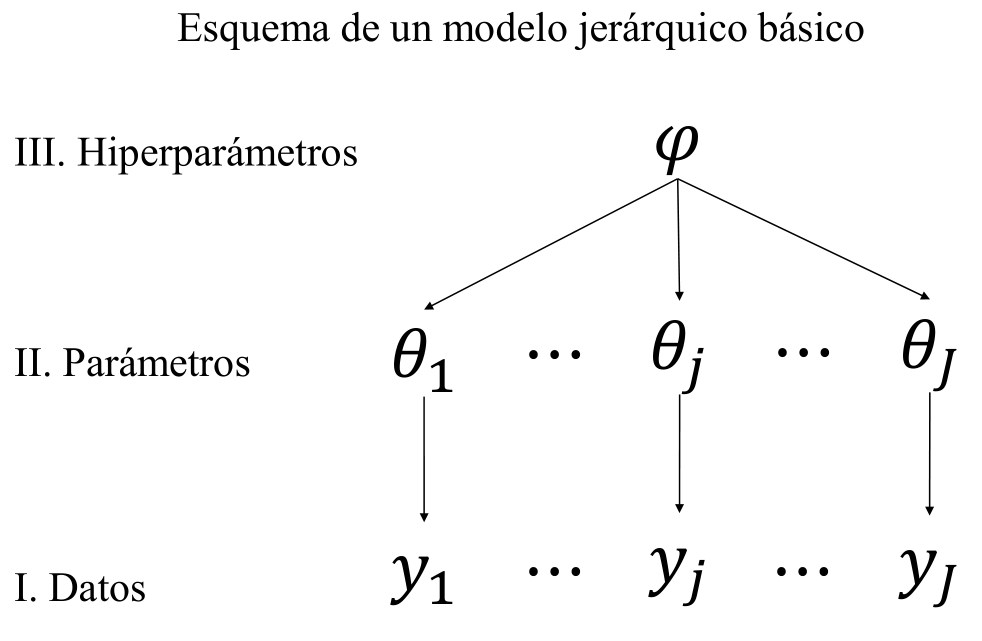
\includegraphics[scale=0.25]{Figs/Bayes/Modelo_Jer}
	\caption{Esquema de un modelo jerárquico básico. Fuente: elaboración propia.}
	\label{fig:Esquema_Modelo_Jer}	
\end{figure}
